\documentclass[11pt]{article}
\usepackage[toc,page]{appendix}
\usepackage{amsmath, amssymb}
\usepackage[utf8]{inputenc}
\usepackage[T1]{fontenc}
\usepackage[style=apa,backend=biber]{biblatex}
\addbibresource{references.bib}
\usepackage{graphicx}
\usepackage{tikz}
\usetikzlibrary{automata,positioning,shapes.geometric, arrows.meta, fit, backgrounds, calc, chains}
\graphicspath{./images/Easy_Pictures/SMR_MULT_Repackaging}
\usepackage{float}
\usepackage[margin=1in]{geometry}
\usepackage{cancel}
\usepackage{epsfig}
\usepackage{tikz-3dplot}
\usepackage{darkmode}
\usepackage{dirtytalk}
\usepackage{longtable,booktabs,array}
\usepackage{calc} % for calculating minipage widths
\usepackage{xcolor}
\usepackage{listings}
\usepackage{etoolbox}
\usepackage{hyperref}
\hypersetup{
 colorlinks=true,
 linkcolor=blue,
 filecolor=magenta, 
 urlcolor=cyan,
 pdftitle={Hermeneutic Calculator},
 citecolor=blue,
}
\urlstyle{same}

\lstdefinestyle{htmlStyle}{
 language=HTML,
 basicstyle=\ttfamily\small,
 keywordstyle=\color{blue}\bfseries,
 commentstyle=\color{gray}\itshape,
 stringstyle=\color{red},
 breaklines=true,
 frame=single,
 numbers=left,
 numberstyle=\tiny\color{gray},
 columns=fullflexible,
}
\lstdefinelanguage{HTML}{
 keywords={<!DOCTYPE, html, head, title, body, h1, h2, h3, p, div, span, a, img, ul, li, table, tr, td, th, style, link, script},
 sensitive=true,
 comment=[l]{//},
 morecomment=[s]{/*}{*/},
 morestring=[b]',
 morestring=[b]"
}
\lstset{style=htmlStyle, language=html}

\definecolor{sliceRed}{RGB}{225,224,91}
\definecolor{linkYellow}{RGB}{255,215,0}
\tdplotsetmaincoords{70}{110}

\title{Strategic Multiplicative Reasoning - Coordinating Two Counts}
\author{Compiled by: Theodore M. Savich}
\date{\today}

\begin{document}
\maketitle

\subsection*{Transcript}
Video from \textcite{Carpenter1999}. Strategy descriptions and examples adapted from \textcite{HackenbergCourseNotes}

\begin{itemize}
      \item \textbf{Teacher:} Jason has three bags of cookies. There are six cookies in each bag. How many cookies does Jason have altogether? 
      \item \textbf{Alex:} There are three bags, right? Six are in each bag. 1, 2, 3, 4, 5, 6. 1, 2, 3, 4, 5, 6. 1, 2, 3, 4, 5, 6. 1, 2, 3, 4, 5, 6, will go in this bag. 1, 2, 3, 4, 5, 6. Six will go into this bag. And 1, 2, 3, 4, 5, 6, will go into this bag. So 1, 2, 3, 4, 5, 6, 7, 8, 9, 10, 11, 12, 13, 14, 15, 16, 17, 18. Eighteen cookies are in each bag
      \item \textbf{Teacher:} Nice, thank you. Put those aside.
\end{itemize}

\noindent 
Alex started by arranging three unifix cubes. Soon, he realized that he needed to count cookies. He initially counted in groups of six cubes, even exceeding three complete groups. Recognizing this approach was inefficient, he began again—this time, he placed one cube to represent a bag and then added six cubes to stand for the cookies that would fill that bag. He repeated this process three times. Finally, by counting all the cubes (each standing in for a cookie), he determined there were 18 cookies in total.

In general, count incrementally by ones, but keep track of how many groups you are counting to coordinate the two distinct types of units involved.

\subsection*{Coordinating Two Counts by Ones (C2C)}

\subsubsection*{Description of Strategy:}
\begin{itemize}
    \item \textbf{Objective:} Count the total number of items by counting each item one by one, while keeping track of both the number of groups and the number of items in each group.
    \item \textbf{Method:} For each group, count the items in that group by ones, and repeat this for each group, incrementing the total count.
\end{itemize}

\subsubsection*{Automaton Type:}
\textbf{Finite State Automaton (FSA)} with counters.

\subsubsection*{Formal Description of the Automaton}

We define the automaton as the tuple
\[
M = (Q,\, \Sigma,\, \delta,\, q_{0/accept},\, F,\, V),
\]
where:
\begin{itemize}
    \item \( Q = \{q_{0/accept},\, q_{\text{count\_items}},\, q_{\text{next\_group}}\} \) is the set of states.
    \item \(\Sigma\) is the input alphabet (used, for example, to read the initial values for the problem).
    \item \(q_{0/accept}\) is the start state, which is also the accept state.
    \item \( F = \{q_{0/accept}\} \) is the set of accepting states.
    \item \( V = \{\text{GroupCounter (G)},\, \text{ItemCounter (I)},\, \text{TotalCounter (T)},\, \text{GroupSize (S)},\, \text{TotalGroups (N)}\} \) is the set of variables.
\end{itemize}

\paragraph{Key Transitions:}
\begin{enumerate}
    \item \textbf{Initialization:} From \(q_{0/accept}\), on reading the input (e.g., the values of \(S\) and \(N\)), set \(G=0\), \(I=0\), and \(T=0\), then move to \(q_{\text{count\_items}}\).
    \item \textbf{Counting Items:} In \(q_{\text{count\_items}}\), for each item in the current group, increment \(I\) and \(T\) (looping until \(I=S\)).
    \item \textbf{Moving to Next Group:} When \(I=S\) (the current group is complete), transition to \(q_{\text{next\_group}}\) where \(G\) is incremented and \(I\) is reset to 0.
    \item \textbf{Completion:} In \(q_{\text{next\_group}}\), if \(G = N\) (all groups have been counted), transition back to \(q_{0/accept}\) to output the total count \(T\); otherwise, return to \(q_{\text{count\_items}}\) for the next group.
\end{enumerate}

\subsubsection*{Automaton Diagram for C2C}

\begin{figure}[H]
\centering
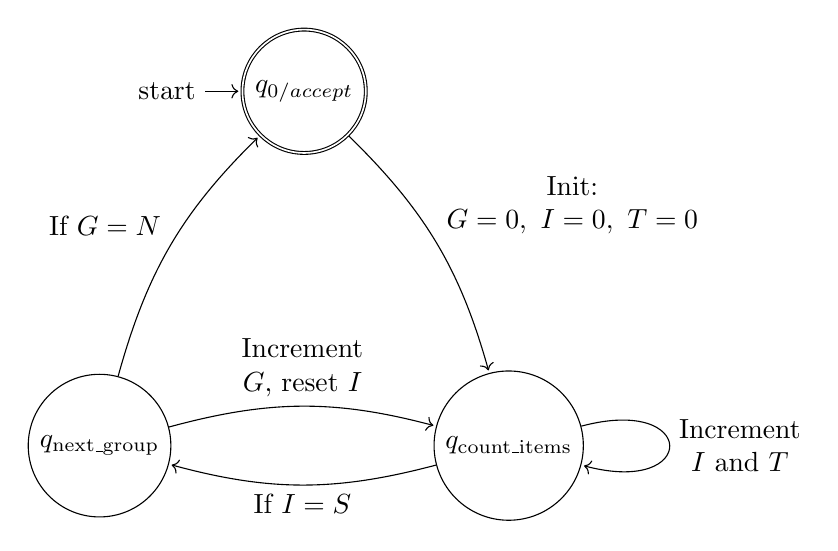
\begin{tikzpicture}[
    shorten >=1pt,
    auto,
    node distance=3cm,
    every state/.style={minimum size=1cm}
]
    \node[state, initial, accepting] (q0) at (90:3cm) {$q_{0/accept}$};
    \node[state] (q1) at (330:3cm) {$q_{\text{count\_items}}$};
    \node[state] (q2) at (210:3cm) {$q_{\text{next\_group}}$};

    \path[->]
        (q0) edge[bend left=15] 
            node[above right, align=center] 
            {Init: \\
             \(G=0,\ I=0,\ T=0\)} 
            (q1)
        (q1) edge[loop right] 
            node[right, align=center] 
            {Increment \\ \(I\) and \(T\)} 
            (q1)
        (q1) edge[bend left=15] 
            node[below, align=center] 
            {If \(I=S\)} 
            (q2)
        (q2) edge[bend left=15] 
            node[above, align=center] 
            {Increment \\ \(G\), reset \(I\)} 
            (q1)
        (q2) edge[bend left=15] 
            node[above left, align=center] 
            {If \(G=N\)} 
            (q0);
\end{tikzpicture}
\caption{FSA with counters to coordinate item and group counting by ones.}
\end{figure}

\subsection*{Extending to a Two-Stack Automaton (2-PDA)}

While the above FSA captures the essence of coordinating two types of counts (items and groups), it does not explicitly illustrate the use of a stack. If one requires \textit{unbounded} counting or more advanced structure (e.g., repeated addition for multiplication in a more formal sense), a single-stack PDA can be designed. However, to \textbf{compose two distinct PDAs}—one for the item count and one for the group count—and retain each one’s push/pop operations, we can move to a \textbf{two-stack pushdown automaton (2-PDA)}. This sort of machine:

\begin{itemize}
    \item Uses two independent stacks, Stack$_1$ and Stack$_2$, each manipulated by transitions in its own sub-automaton.
    \item Has states that combine the “local states” of the separate PDAs. A state in the 2-PDA is effectively a pair \((q_1, q_2)\), where \(q_1\) is from the item-counting PDA and \(q_2\) is from the group-counting PDA.
    \item Pushes and pops symbols from either (or both) stacks, depending on which sub-automaton’s transition is activated.
\end{itemize}

\subsubsection*{Formal 2-PDA Composition}

Let:
\[
P_1 = (Q_1,\ \Sigma,\ \Gamma_1,\ \delta_1,\ q_{1,0},\ F_1)
\quad\text{and}\quad
P_2 = (Q_2,\ \Sigma,\ \Gamma_2,\ \delta_2,\ q_{2,0},\ F_2)
\]
be two PDAs (each with its own stack alphabet, \(\Gamma_1\) and \(\Gamma_2\), and transition functions \(\delta_1\) and \(\delta_2\)). The \textbf{two-stack automaton} \(P_{\times}\) that composes them is:

\[
P_{\times} = 
\bigl(Q_1 \times Q_2,\ 
\Sigma,\ 
\Gamma_1,\ 
\Gamma_2,\ 
\delta_{\times},\ 
(q_{1,0}, q_{2,0}),\ 
F_1 \times F_2\bigr),
\]
where
\[
\delta_{\times}\bigl((q_1,q_2),\,a,\,X,\,Y\bigr) = 
\bigl\{
    \bigl((q_1',q_2'),\ \alpha,\ \beta\bigr)
    \,\big|\,
    (q_1', \alpha) \in \delta_1(q_1,\,a,\,X)\ \text{and}\ (q_2', \beta) \in \delta_2(q_2,\,\epsilon,\,Y)
\bigr\},
\]
and similarly for transitions where \(P_2\) processes input \(a\) while \(P_1\) processes \(\epsilon\). The notation means:
\begin{itemize}
    \item On input symbol \(a\), with the top of Stack$_1$ being \(X\) and the top of Stack$_2$ being \(Y\), the composite automaton transitions to \((q_1',q_2')\).
    \item It replaces \(X\) with \(\alpha\) in Stack$_1$ (possibly pushing or popping multiple symbols) and \(Y\) with \(\beta\) in Stack$_2$.
\end{itemize}

\paragraph{Interpreting the Two Stacks for Multiplication}
- \textbf{Stack$_1$}: Manages the state of counting items in one group (similar to your single-stack counting idea, but restricted to item-level detail).  
- \textbf{Stack$_2$}: Manages the state of counting how many groups have been multiplied so far (e.g., for repeated addition).

During each “repeated addition” cycle:
1. The item-counting sub-automaton (PDA$_1$) increments the partial total by the group size, pushing/popping from Stack$_1$.
2. The group-counting sub-automaton (PDA$_2$) tracks how many times this addition has been done, pushing/popping from Stack$_2$.

Once PDA$_2$ indicates all groups have been accounted for, the 2-PDA halts or transitions to an accepting state.

\subsection*{Example of Counting Three Groups of Six (High-Level 2-PDA)}

\begin{enumerate}
    \item \textbf{Stacks Initialization:} 
    \begin{itemize}
        \item Stack$_1$ starts with the necessary markers/symbols to begin item counting.
        \item Stack$_2$ starts with a symbolic representation of how many groups remain (e.g., 3).
    \end{itemize}
    \item \textbf{Item Counting Process (Stack$_1$):} 
    \begin{itemize}
        \item Each time the automaton processes the addition of 6 items to the partial total, it pushes/pops in Stack$_1$ to record digits in base-\(b\) or some other scheme.
    \end{itemize}
    \item \textbf{Group Countdown (Stack$_2$):}
    \begin{itemize}
        \item After finishing one addition cycle for 6 items, pop one “group token” from Stack$_2$. 
        \item If Stack$_2$ is not empty, move on to add another 6.
        \item If Stack$_2$ becomes empty, the multiplication is complete.
    \end{itemize}
\end{enumerate}

\paragraph{Why a 2-PDA?}
Composing two separate single-stack PDAs \textit{in parallel} effectively yields a machine with two stacks. The 2-PDA formalism lets each “sub-automaton” maintain its independent pushdown memory, which can be advantageous if you conceptually want to keep the logic of item-counting and group-counting separate. In theoretical terms, a 2-PDA is already as powerful as a Turing machine, so it can handle the entire repeated-addition multiplication process without additional resources.

\subsection*{Conclusion on the Two-Stack Approach}

Using a two-stack automaton is a straightforward way to \textbf{combine} two independently designed PDAs so that each retains its own stack-based memory management. This might be done for instructional clarity or for theoretical completeness when demonstrating that distinct counting mechanisms can be kept separate. In practice, a single-stack PDA can also implement multiplication by carefully interleaving the logic in one stack. However, splitting the tasks across two separate stacks can simplify the conceptual breakdown of item counting versus group counting.


\clearpage
\subsubsection*{HTML Implementation}
\lstinputlisting[style=htmlStyle, language=html]{./new_html/SMR_Multiplication_Coordinating_Two_Counts.html}


\printbibliography

\end{document}
